\chapter{Visualization}

%%%%%%%%%%%%%%%%%%%%%%%%%%%%%%%%%%%%%%%%%%%%%%%
% Progression Bar
% |===================>|
% empty chapter        chapter finished
%%%%%%%%%%%%%%%%%%%%%%%%%%%%%%%%%%%%%%%%%%%%%%%

Visualizing data on a non-regular grids is a task on its own, because the number of tools for solving such problem is very limited. NCL is one of them and we chose it as the main tool for ICON. You can find several examples of how to write simple plot scripts for ICON data sets on this website: \href{http://www.ncl.ucar.edu/Applications/icon.shtml}{http://www.ncl.ucar.edu/Applications/icon.shtml}. The coordinate information is essential for writing your own plot scripts. ICON output files currently have three different types of them: cells, edges and vertices, e.g. tracers like temperature and salinity and surface elevation are defined on each cell center while the normal velocity is defined on edges.

\section{icon\_plot.ncl}

For getting around the different coordinates and in order not to rewrite things there is a general plot scripts: {\tt icon\_plot.ncl}. It supports contour and vector plots, a combination of both via overlaying and vertical sections. Both atmosphere and ocean vertical coordinate systems can be handled by it: While ocean uses a plain depth axes, atmosphere model uses hybrid sigma pressure levels (hydrostatic) and free 3D height variable (non-hydrostatic).

The script {\tt icon\_plot.ncl} is a single NCL program, which provides multiple plot types for data on ICON's grid. It is located in the ICON-repository under \\
{\tt source:/trunk/icon-dev/scripts/postprocessing/tools/icon\_plot.ncl}. Most of the functionality is implemented in a library: {\tt icon\_plot\_lib.ncl} located in \\
{\tt source:/trunk/icon-dev/scripts/postprocessing/tools/icon\_plot\_lib.ncl}. Both files are installed into the {\tt /pool/data/ICON/tools} which is the default lookup location for the library. For different location like an icon checkout, use altLibDir, e.g. \\
{\tt altLibDir='"/home/user/src/icon-dev/tools"'}.

\subsection{Requirements}
\begin{itemize}
\item NCL 5.2.1 is the minimum version of NCAR's plotting language (\href{http://www.ncl.ucar.edu}{http://www.ncl.ucar.edu})
\item CDO (\href{https://code.zmaw.de/projects/cdo}{https://code.zmaw.de/projects/cdo})
\end{itemize}

\subsection{Customization}
{\tt icon\_plot.ncl} optionally reads a configuration file named {\tt \$HOME/.icon\_plot.rc} where default options can be set. Actually it is handled like an ordinary ncl file. This can be used to customize the {\tt altLibDir} setting, e.g.:

\begin{small}
\begin{verbatim}
altLibDir="/home/ram/src/git/icon/scripts/postprocessing/tools" 
oType="png" 
\end{verbatim}
\end{small}

\subsection{Basic command line option}
Required are options for
\begin{enumerate}
\item \textbf{Input/output files}: Use the variable {\tt iFile} for defining the input and {\tt oFile} for the output file. It's extension depends on the output type, which can be set with {\tt oType}. If {\tt oFile} is left out, the output file will inherit its name from the input file.
\item \textbf{Variable selection}: Depending on the plot mode you like to use, {\tt varName} for scalar variables or {\tt vecVars} for vector-variables must be uses.
\end{enumerate}

Optional (default:0) parameter are
\begin{enumerate}
\item \textbf{Level selection}: Levels can only be selected by their index. That's why, the corresponding variables is called {\tt levIndex}. Please note that it starts with 0, like any other NCL indices.
\item \textbf{Time selection}: Like levIndex, the variable {\tt timeStep} can be used to select a certain time step, again starting from 0.
\end{enumerate}

There are many more parameters (see \ref{all_options}) for mapping, transections, selecting regions and masking, but these are the most fundamental ones.

\subsection{Plot Types}
For flexibility the selection of a specific plot mode is implemented by combining certain options.

\subsubsection{Contour plots}
Contour plot are the default plot mode. If only the require parameters are set, e.g. {\tt iFile} and {\tt varName}, a simple contour plot is created with

\begin{small}
\begin{verbatim}
ncl icon_plot.ncl 'varName="T"' 'iFile="iFILENAME"'
\end{verbatim}
\end{small}

This is a basic temperature plot. Captions are set to basic information like variable name, time and level information and input filename.

\begin{figure}[h!]%
\centering
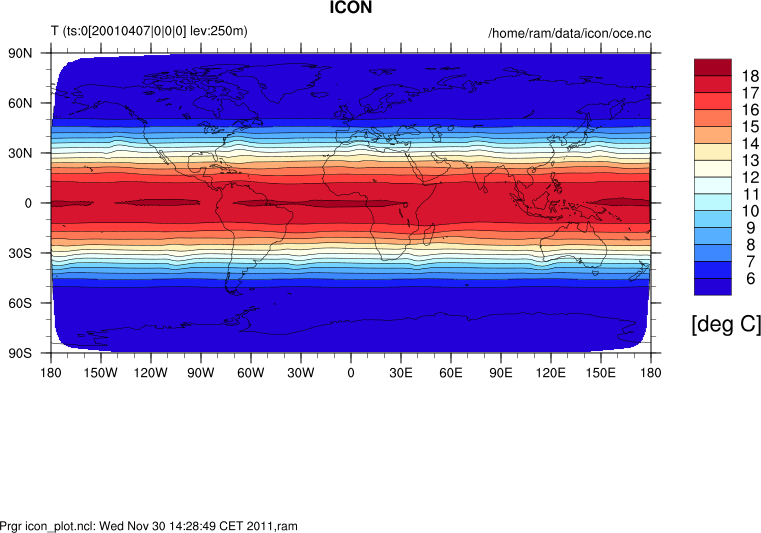
\includegraphics[width=0.95\linewidth]{pictures/contour_plot.png}
\caption{Example of contour plot}\label{fig:contour-plot}
\end{figure}

\subsubsection{Vector plots}
Use {\tt vecVars} instead of {\tt varName}. To adjust the length of the reference vector, use the variable {\tt vecRefLength}.

\begin{small}
\begin{verbatim}
ncl icon_plot.ncl 'vecVars="U V"' 'iFile="iFILENAME"' vecRefLength=0.01
\end{verbatim}
\end{small}

\begin{figure}[h!]%
\centering
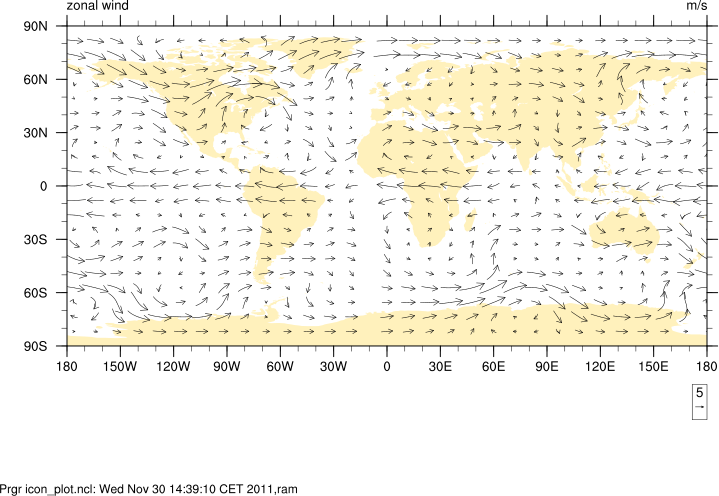
\includegraphics[width=0.95\linewidth]{pictures/vector_plot.png}
\caption{Example of vector plot}\label{fig:vector-plot}
\end{figure}

\subsubsection{Overlay of scalar and vector variables}
Contour and vector plots can be combined into a single plot by overlaying both. Following this approach, such an overlay plot will be created, if {\tt varName} and {\tt vecVars} are given: 

\begin{small}
\begin{verbatim}
ncl icon_plot.ncl 'varName="T"' 'iFile="iFILENAME"' 'vecVars="U V"'
\end{verbatim}
\end{small}

\begin{figure}[h!]%
\centering
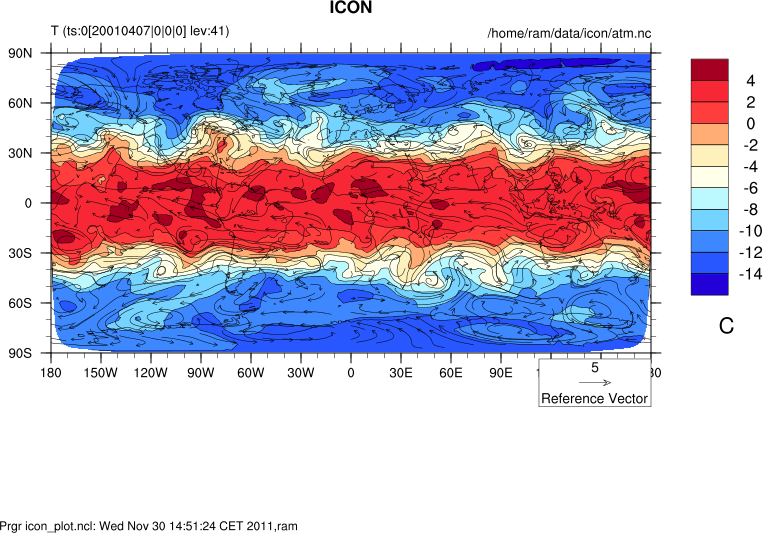
\includegraphics[width=0.95\linewidth]{pictures/overlay_plot.png}
\caption{Example of overlay plot}\label{fig:overlay-plot}
\end{figure}

\subsubsection{Vertical sections}
Data for sections have to be interpolated first. This is done internally and you do not have to care about it. Section plot are created, if a start and and end point of a section is given. For this purpose, the variables {\tt secLC} (section-left-corner) and {\tt secRC} (section-right-corner) have to be used. Theses variable have to be {\tt (lon,lat)} arrays like {\tt secLC=(/20.,30./)}.

Example call:

\begin{small}
\begin{verbatim}
ncl icon_plot.ncl 'varName="T"' 'iFile="iFILENAME"'  \
    'secLC=(/0,80/)' 'secRC=(/0,-80/)'
\end{verbatim}
\end{small}

{\tt secPoints} is an option to set the accuracy of the plot. The representing of the location of the section is suppressed by setting {\tt showSecMap=False}. Its default value is {\tt True}.

\begin{figure}[h!]%
\centering
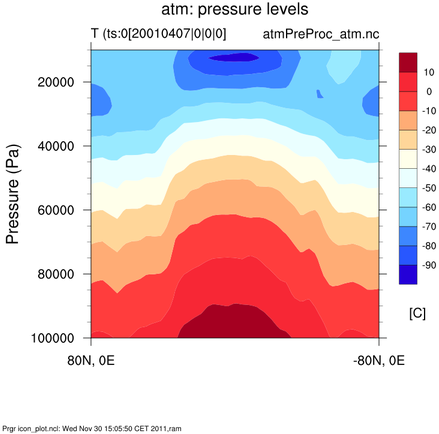
\includegraphics[width=0.95\linewidth]{pictures/vertsection_plot.png}
\caption{Example of vertical sections plot}\label{fig:vertsections-plot}
\end{figure}

\subsubsection{Display the ICON grid}
Set the parameter {\tt showGrid} to {\tt True} and for scalar variables, the ICON grid is represented instead of the contour plot. For large grids, this can take a long time.

\subsection{Regional plots}
Use the variables {\tt mapLLC} (map-Lower-Left-Corner) and {\tt mapURC} (map-Upper-Right-Corner) to select special regions of the earth. Here is a list of useful examples:

\begin{table}[htd]
\caption{Examples of useful regional plots}
\begin{center}
\begin{tabular}{lll}\hline
Trop. Atlantic &	{\tt 'mapLLC=(/-60, -25/)'}	& {\tt 'mapURC=(/ 25,25/)'}\\
North Polar	&{\tt 'mapLLC=(/-200, 20/)'}	& {\tt 'mapURC=(/160,90/)'}\\
North Atlantic	&{\tt 'mapLLC=(/-100,-15/)'}	& {\tt 'mapURC=(/ 35,65/)'}\\
Labrador/Panama	&{\tt 'mapLLC=(/-200, -5/)'}	 &{\tt 'mapURC=(/ 35,85/)'}\\
North Atlantic/Eurasia&	{\tt 'mapLLC=(/ -80, -5/)'}&	 {\tt 'mapURC=(/ 75,85/)'}\\
Asia	&{\tt 'mapLLC=(/ 20,-15/)'}	& {\tt 'mapURC=(/160,85/)'}\\\hline
\end{tabular}
\end{center}
\end{table}

\newpage

\subsection{Masking}
Masking can be done in two different ways:
\begin{enumerate}
\item Manually mask the data with CDO before running the plot scripts, i.e. use the ifthen operator or perform a division with the mask variable:
\begin{small}
\begin{verbatim}
 cdo div iconInput.nc -selname,mask_variable iconInput.nc maskedOutput.nc
\end{verbatim}
\end{small}
\item Let the plot script perform the masking using the NCL's mask function. For this purpose, the commandline variables {\tt maskName} and {\tt maskFile} have to be used. If the mask variable is part of the regular input file, {\tt maskFile} can be left out.
\end{enumerate}

Both methods have their pros and cons. Whereas the second methods works fine for all types of horizontal representation, the first produces better results for vertical cross sections.

\subsection{Data on other grids}
Although {\tt icon\_plot.ncl} is implemented for ICON, it can be used for data an regular grids, too. In this case, internal interpolation is not performed.

\subsection{All options}\label{all_options}
{\tt icon\_plot.ncl} has built-in documentation of all options. Use
\begin{small}
\begin{verbatim}
ncl icon_plot.ncl help=True 
\end{verbatim}
\end{small}

%MORE INFORMATION IN REDMINE!!!! (including graphics etc., ask Daniel for access)

\section{ncview/GrADS}
Ncview (\href{http://meteora.ucsd.edu/~pierce/ncview_home_page.html}{http://meteora.ucsd.edu/\~{}pierce/ncview\_home\_page.html}) and GrADS (\href{http://www.iges.org/grads/}{http://www.iges.org/grads/}) can be used after converting icon data sets to a regular grid. This can easily be done with cdo:
\begin{small}
\begin{verbatim}
cdo -P 8 -r remapnn,r180x90 icon.nc regular_icon.nc
\end{verbatim}
\end{small}
This uses nearest neighbor interpolation and hereby keeps the model values. When using a higher regular resolution the triangular icon grid keeps visible.

\section{Other Possibilities}
\begin{itemize}
\item GMT is useful, when the grid should be visualized.
\item ParaView is an alternative to display data on an unstructured grid. As a caveat, the model output has first to be converted into the vtk format.
\end{itemize}


\newpage
\subsection*{Discussion}

%This sction is for discussion only. Please add your notes, your name and date.
%Document last edited by \textit{Daniel Rieger} on \textit{26.11.2013}.\\
Document last edited by \textit{\krauti} on \textit{29.11.2013}.\\
Note: -
